\documentclass{article}\usepackage[]{graphicx}\usepackage[]{color}
%% maxwidth is the original width if it is less than linewidth
%% otherwise use linewidth (to make sure the graphics do not exceed the margin)
\makeatletter
\def\maxwidth{ %
  \ifdim\Gin@nat@width>\linewidth
    \linewidth
  \else
    \Gin@nat@width
  \fi
}
\makeatother

\definecolor{fgcolor}{rgb}{0.345, 0.345, 0.345}
\newcommand{\hlnum}[1]{\textcolor[rgb]{0.686,0.059,0.569}{#1}}%
\newcommand{\hlstr}[1]{\textcolor[rgb]{0.192,0.494,0.8}{#1}}%
\newcommand{\hlcom}[1]{\textcolor[rgb]{0.678,0.584,0.686}{\textit{#1}}}%
\newcommand{\hlopt}[1]{\textcolor[rgb]{0,0,0}{#1}}%
\newcommand{\hlstd}[1]{\textcolor[rgb]{0.345,0.345,0.345}{#1}}%
\newcommand{\hlkwa}[1]{\textcolor[rgb]{0.161,0.373,0.58}{\textbf{#1}}}%
\newcommand{\hlkwb}[1]{\textcolor[rgb]{0.69,0.353,0.396}{#1}}%
\newcommand{\hlkwc}[1]{\textcolor[rgb]{0.333,0.667,0.333}{#1}}%
\newcommand{\hlkwd}[1]{\textcolor[rgb]{0.737,0.353,0.396}{\textbf{#1}}}%
\let\hlipl\hlkwb

\usepackage{framed}
\makeatletter
\newenvironment{kframe}{%
 \def\at@end@of@kframe{}%
 \ifinner\ifhmode%
  \def\at@end@of@kframe{\end{minipage}}%
  \begin{minipage}{\columnwidth}%
 \fi\fi%
 \def\FrameCommand##1{\hskip\@totalleftmargin \hskip-\fboxsep
 \colorbox{shadecolor}{##1}\hskip-\fboxsep
     % There is no \\@totalrightmargin, so:
     \hskip-\linewidth \hskip-\@totalleftmargin \hskip\columnwidth}%
 \MakeFramed {\advance\hsize-\width
   \@totalleftmargin\z@ \linewidth\hsize
   \@setminipage}}%
 {\par\unskip\endMakeFramed%
 \at@end@of@kframe}
\makeatother

\definecolor{shadecolor}{rgb}{.97, .97, .97}
\definecolor{messagecolor}{rgb}{0, 0, 0}
\definecolor{warningcolor}{rgb}{1, 0, 1}
\definecolor{errorcolor}{rgb}{1, 0, 0}
\newenvironment{knitrout}{}{} % an empty environment to be redefined in TeX

\usepackage{alltt}
\IfFileExists{upquote.sty}{\usepackage{upquote}}{}
\begin{document}

\begin{knitrout}
\definecolor{shadecolor}{rgb}{0.969, 0.969, 0.969}\color{fgcolor}\begin{kframe}
\begin{alltt}
\hlcom{#======================================================================}
\hlcom{#graph for hw 2 - number 1}
\hlcom{#}
\hlcom{# Tyler Bradley}
\hlcom{# 1/28/2018}
\hlcom{#======================================================================}
\end{alltt}
\end{kframe}
\end{knitrout}

Loading required libraries

\begin{knitrout}
\definecolor{shadecolor}{rgb}{0.969, 0.969, 0.969}\color{fgcolor}\begin{kframe}
\begin{alltt}
\hlkwd{library}\hlstd{(tidyverse)}
\hlkwd{library}\hlstd{(broom)}
\end{alltt}
\end{kframe}
\end{knitrout}

Creating dataset from problem

\begin{knitrout}
\definecolor{shadecolor}{rgb}{0.969, 0.969, 0.969}\color{fgcolor}\begin{kframe}
\begin{alltt}
\hlstd{ffa_data} \hlkwb{<-} \hlkwd{tribble}\hlstd{(}
  \hlopt{~}\hlstd{t,}   \hlopt{~}\hlstd{c_ffa,}
  \hlnum{0}\hlstd{,}     \hlnum{4e-5}\hlstd{,}
  \hlnum{10}\hlstd{,}    \hlnum{2.43e-5}\hlstd{,}
  \hlnum{20}\hlstd{,}    \hlnum{1.48e-5}\hlstd{,}
  \hlnum{30}\hlstd{,}    \hlnum{8.98e-6}\hlstd{,}
  \hlnum{40}\hlstd{,}    \hlnum{5.46e-6}\hlstd{,}
  \hlnum{50}\hlstd{,}    \hlnum{3.32e-6}\hlstd{,}
  \hlnum{60}\hlstd{,}    \hlnum{2.02e-6}
\hlstd{)} \hlopt
  \hlcom{# adding ln(C_ffa) column}
  \hlcom{# log() function in R defaults to ln}
  \hlkwd{mutate}\hlstd{(}\hlkwc{ln_c_ffa} \hlstd{=} \hlkwd{log}\hlstd{(c_ffa))}
\end{alltt}
\end{kframe}
\end{knitrout}

Plotting the log concentration of FFA vs time

\begin{knitrout}
\definecolor{shadecolor}{rgb}{0.969, 0.969, 0.969}\color{fgcolor}\begin{kframe}
\begin{alltt}
\hlkwd{ggplot}\hlstd{(ffa_data,} \hlkwd{aes}\hlstd{(t, ln_c_ffa))} \hlopt{+}
  \hlkwd{geom_point}\hlstd{()} \hlopt{+}
  \hlkwd{geom_smooth}\hlstd{(}\hlkwc{method} \hlstd{=} \hlstr{"lm"}\hlstd{)} \hlopt{+}
  \hlkwd{theme_bw}\hlstd{()}
\end{alltt}
\end{kframe}
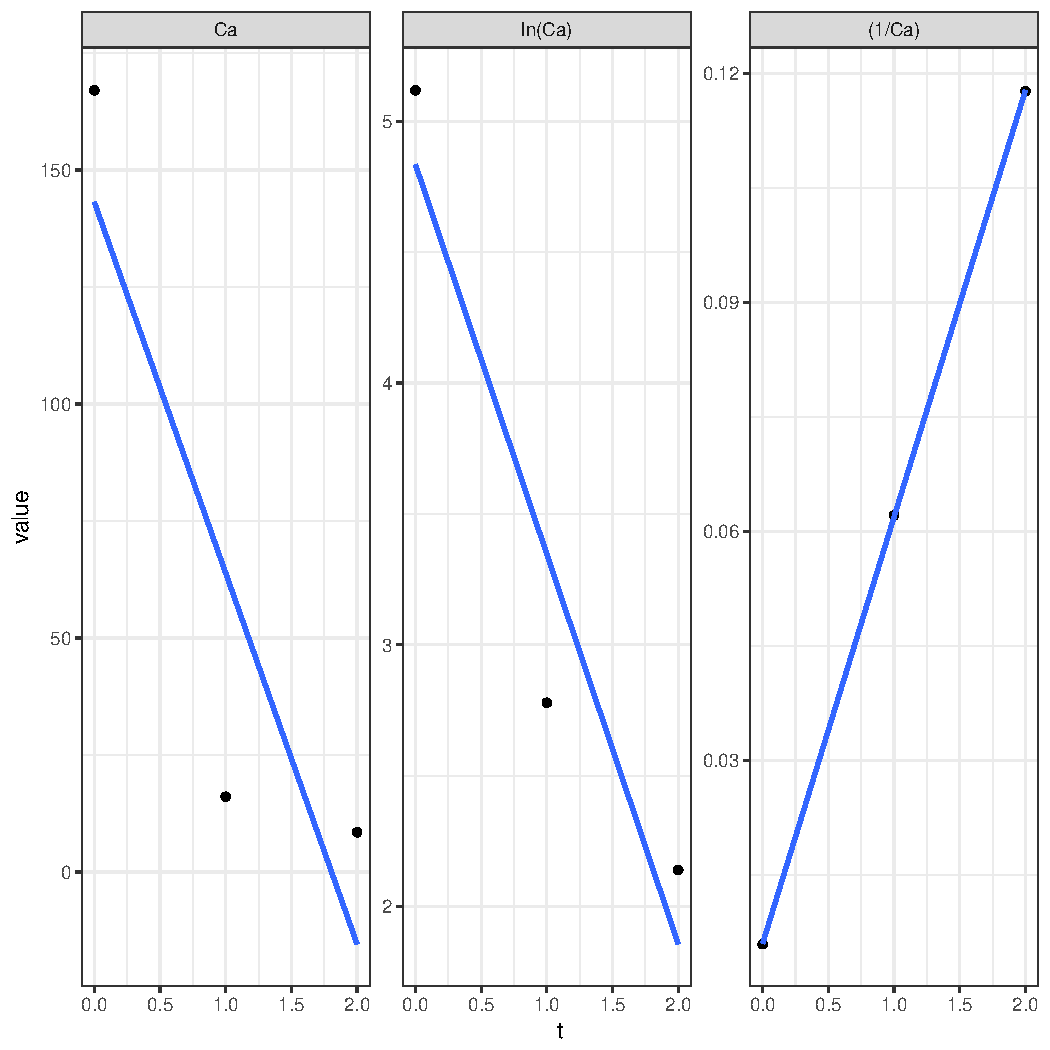
\includegraphics[width=\maxwidth]{figure/unnamed-chunk-4-1} 

\end{knitrout}

Running linear model to get slope and intercept values.

\begin{knitrout}
\definecolor{shadecolor}{rgb}{0.969, 0.969, 0.969}\color{fgcolor}\begin{kframe}
\begin{alltt}
\hlstd{ffa_model} \hlkwb{<-} \hlstd{ffa_data} \hlopt
  \hlkwd{nest}\hlstd{()} \hlopt
  \hlkwd{mutate}\hlstd{(}\hlkwc{lm_model} \hlstd{=} \hlkwd{map}\hlstd{(data,} \hlopt{~}\hlkwd{lm}\hlstd{(ln_c_ffa} \hlopt{~} \hlstd{t,} \hlkwc{data} \hlstd{= .x)),}
         \hlkwc{lm_tidy} \hlstd{=} \hlkwd{map}\hlstd{(lm_model, tidy))}

\hlcom{# Printing linear model coeffecients.}
\hlstd{ffa_model} \hlopt \hlkwd{unnest}\hlstd{(lm_tidy,} \hlkwc{.drop} \hlstd{=} \hlnum{TRUE}\hlstd{)} \hlopt \hlstd{knitr}\hlopt{::}\hlkwd{kable}\hlstd{()}
\end{alltt}
\end{kframe}
\begin{tabular}{l|r|r|r|r}
\hline
term & estimate & std.error & statistic & p.value\\
\hline
(Intercept) & -10.1267742 & 0.0005306 & -19087.002 & 0\\
\hline
t & -0.0497698 & 0.0000147 & -3382.239 & 0\\
\hline
\end{tabular}


\end{knitrout}

\end{document}
